\documentclass{article}
\usepackage[utf8]{inputenc}
\usepackage{diffcoeff}  
\usepackage{amsmath}
\usepackage{amssymb}
\usepackage{cancel}
\usepackage{nicefrac}
\usepackage{graphicx}
\usepackage{geometry}
\geometry{letterpaper, top=25mm, bottom=25mm, left=25mm, right=25mm}


\title{Modelling The Flow of Crowds}

\begin{document}
\maketitle

\section{Introduction}
(...)
Two fundamental frameworks have been proposed to model crowd motion. The first treats pedestrians as discrete individuals, allowing for a great deal of flexibility and precision in defining each person's behaviour. Generally, a computer simulation is used to simulate the crowd under a specific set of circumstances. This model is best suited to small, less dense clusters of people, and lacks the ability to provide us with general results on crowd behaviour. Conversely, the second framework, analyzed in this paper, observes the crowd as a whole and treats it like a continuum. The individuals involved all follow the same general behavioural pattern, moving as efficiently as possible to reach their objectives. This makes it better suited to larger, denser crowds, whose behaviour approximate a continuum.

\section{Derivation}
\subsection{Physical Assumptions}
\newcommand\Rpix{\mathcal R_{\text{\texttt{px}}}}
\newcommand{\brydon}{\texttt{Brydon}}
In order to go about modelling something as complex as a group of human individuals, we must make a few simplifying assumptions. Let $\mathcal R\subseteq\mathbb R^2$ be an arbitrary region in space with a smooth boundary, where the crowd operates. Firstly, we must assume that the crowd is dense enough that its behaviour mimics a continuum, or our model will be inaccurate. In other words, there are enough people per unit area such that $\mathcal R$ is a nonempty, compact, and connected space. We also assume there are no inanimate obstacles in the crowd large enough to significantly affect the overall flow of people. Finally, we restrict the crowd to operating in only 2 spatial dimensions. Physically, this means that the ground on which the crowd operates is approximately flat, and that people remain close enough to the ground. Hence, our overall model will have 3 independent variables: $x$, $y$ (spatial), and $t$ (temporal).

\subsection{Conservation of Pedestrians}
We start by assuming that in a given area of the crowd, the flow of the pedestrians is conserved. Then, we can set up the skeleton of our PDE by using the conservation law. 

1) Based on the assumption of the crowd acting as a continuum, we can define $\rho$, the density of the "flow" of pedestrians per unit area, at a given time t.

2)This flow of pedestrians would also have a  velocity $\vec{v}$ (in directions x,y) at a given time, at a given location.

3) For our purposes, we will also assume that there is no creation nor destruction of pedestrians.

Therefore, through divergence theorem, we get the following PDE:

\[
    \diffp \rho t = - \nabla\cdot (\rho\vec v)
\]



\subsection{Modelling Behaviour}
In this section, we define the basic behaviour of pedestrians to give their movement a necessary degree of predictability. The following 3 hypotheses frame this behaviour:
\begin{enumerate}
    \item \textbf{Hypothesis 1:} The speed at which any individual pedestrian will walk depends only on the density and behaviour of their surroundings. In other words, under a particular set of circumstances, any individual from the crowd will move at the same speed.
    \\
    This hypothesis defines that for our conservation law, we can have that velocity function is only a function of $\rho$.
    \begin{equation}
        \vec{v} = v(\rho) \hat{v}\label{hyp1}
    \end{equation}
    
    
    \item \textbf{Hypothesis 2:} Each individual has a 'goal' (referred to as 'potential'), or a place they want to get to. We can model this by assigning a 'potential' $\phi(\vec x)$ to each location $\vec x \in\mathcalR \mathbb R^2$. We assume that each person moves to minimize their potential as efficiently as possible. This leads to the following equation,  which tells us how individuals choose their direction of movement.
    \\
    Mathematically speaking, minimizing the potential means moving perpendicular to the "potential", which determines our direction vector as the normal vector to the potential function:
    \begin{equation}
         \hat{v} = \hat{n} = -\frac{\nabla\phi(\vec x)}{\|\nabla\phi(\vec x)\|}
    \end{equation}
    
    
    \item \textbf{Hypothesis 3:} Pedestrians seek to minimize their travel time, while avoiding highly dense clusters of people. The Triangle Inequality tells us that the quickest way to get from point A to point B is to travel in a straight line. In this scenario, individuals abide by this principle, while also taking small detours to avoid highly dense areas in the crowd. To describe this individual path, we will introduce a proportionality factor $g(\rho)$, which accounts for these detours.
    
    - distance between potentials = ....
    
    
    putting it all together:
    
    final equation
    
    
    
    
\end{enumerate}

\section{Stability of the Front}
The PDE derived in the previous section has the potential to model many situations in the real world. From the annual Muslim Hajj to marathons that take place around the world. An interesting historical application is modelling the Battle of Agincourt.

\subsection{The Battle of Agincourt}
The Battle of Agincourt took place on October 25th, 1415 in France. It was between an English army under the control of Henry V and a French-Burgundian army under Charles VI. While details of the battle vary, modern accounts suggest the English had around 6000 to 7000 soldiers. Many soldiers were also weakened by illness and hunger due to previous battles. Comparatively, the French army had 2 lines of 8000 soldiers in each one. Along with around 9000 other soldiers. \\
\\
The battle ended with the English army's victory and a slain French ``wall of bodies" by modern accounts. Reportedly, 6000 French soldiers were dead and 3000 captive. Given the immensely greater and stronger French side, naturally one would assume it would be the French's victory.\\
\\
To explore the events that took place at the front lines, researchers Clements and Hughes (2004) used the equation derived for the flow of crowds to model the behaviour.\\
\\
To set up the physical situation, the battle occurred between two woods around one kilometre apart. The armies themselves began around a kilometre apart from one another. Clements and Hughes denoted $\eta(x,t)$ as the line between the French forces coming from the North and the English from the south as seen in Figure 1. \\
\begin{figure}[h]
\caption{Battle of Agincourt}
\centering
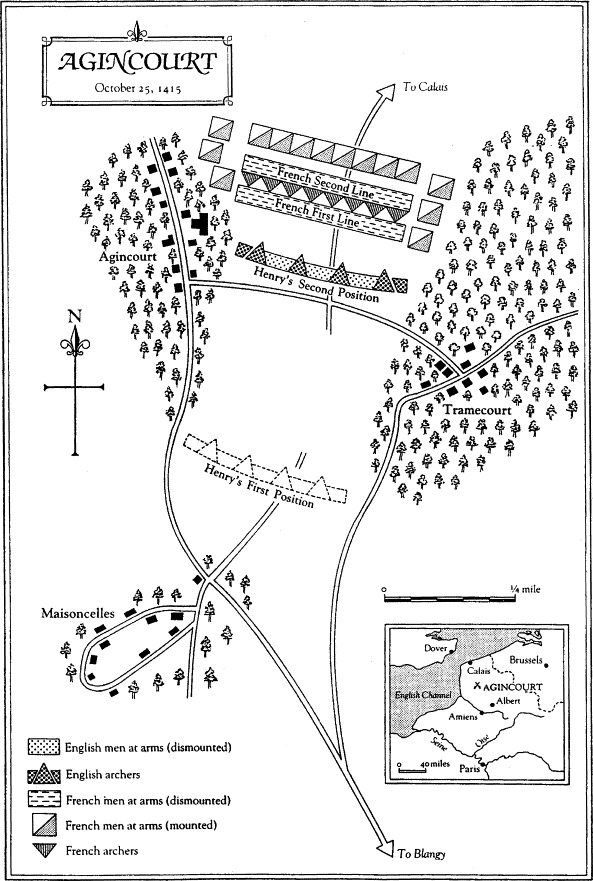
\includegraphics[width=0.5\textwidth]{battlefield.jpg}
\end{figure}
\\
In order to use the PDE the physical assumptions described in section 2 were applied to the soldiers. That is, the researchers assumed a conservation of soldiers and applied the three hypotheses as well. Then using the model they analyzed the stability of the battle front $\eta(x,t)$ using a technique known as ``perturbation series". Furthermore, in the process of doing so, they came upon a description of the battle consistent with first hand accounts however inconsistent with modern popular accounts.

\subsection{A Brief Introduction to Perturbation Series}
One of the main things that Clements and Hughes sought to study was the stability of the front between the French and English soldiers $\eta$. This was achieved using a very powerful technique called ``perturbation series". Though the full extent of how perturbation series were used to find the stability of $\eta$ is beyond the scope of this course, we can demonstrate a simpler example to give an overview of how the technique is used. Consider the problem of finding $\sqrt{4.01}$. Though it may initially seem like we are just complicating things further by doing this, an equivalent problem is finding $a_0,a_1,...\in\mathbb R$ such that
\[
    (a_0+a_1\varepsilon+a_2\varepsilon^2+\cdots)^2=4+\varepsilon
\]
where $\varepsilon=0.01$. In either case, an exact solution is difficult, but an approximate solution is staring us in the face. If we simply round $\varepsilon$ down to zero, then the problem becomes the trivially easy polynomial $a_0^2=4$, which we know the positive solution to be $a_0=2$. In order to improve our approximation, we will need to relax the assumption that $\varepsilon=0$, but we don't necessarily need to get so ambitious as to assume $\varepsilon^2\ne 0$ just yet. After all, $\varepsilon^2$ is quite a bit smaller than $\varepsilon$, and $\varepsilon^3$ is smaller still. If we do this, we get
\begin{align*}
    &(2+a_1\varepsilon)^2=4+\varepsilon\\
    \implies& 4+4a_1\varepsilon+\cancel{a_1^2\varepsilon^2}=4+\varepsilon\\
    \implies& 4a_1\varepsilon=\varepsilon\\
    \implies& (4a_1-1)\varepsilon =0\\
    \implies& a_1=\nicefrac{1}{4}
\end{align*}
This gives us a first order approximation of the solution
\[
    \sqrt{4+0.01}\approx 2+\frac 14(0.01)=2.0025
\]
For reference, plugging the problem into a calculator produces $\sqrt{4.01}\approx 2.00249843945$, so $2.0025$ is already a pretty reasonable approximation. But if we want to go further, we can relax things a bit more, and only round $\varepsilon^n$ for $n>2$. In this case we get
\begin{align*}
    &
    (2+a_1\varepsilon+a_2\varepsilon^2)^2=4+\varepsilon
    \\\implies&
    \cancel{(4a_1-1)}\varepsilon+(a_1^2+2a_2)\varepsilon^2+\cancel{O(\varepsilon^3)}=0
    \\\implies&
    a_2=-\frac 12 a_1^2=-\frac 12 \times \frac 1{16}=-\frac 1{32}
\end{align*}
And hence our second order approximation is
\[
    \sqrt{4.01}\approx 2.002496875
\]
which is in fact closer than the first order approximation. We can continue like this indefinitely until we are satisfied. A useful byproduct of using this technique is that we actually have a general solution to the value of $\sqrt{4+\varepsilon}$ for $\varepsilon\le 1$. Namely
\[
    \sqrt{4+\varepsilon}=2+\tfrac 14\varepsilon-\tfrac 1{32}\varepsilon^2+O(\varepsilon^3)
\]
which tells us something that in this case, we are already well-aware of, but in other cases might not be so obvious. $\sqrt{4+\varepsilon}$ is very likely greater than $\sqrt{4}$ (that is, unless something very bizarre happens for $a_3,a_4,...$). This makes perturbation series a valuable tool for stability analysis. With this in mind, consider the differential equation
\[
    y'=\sqrt y-2
\]
which has one steady-state at $y=4$. Is that steady state stable? Our second order approximation of $\sqrt{4+\varepsilon}$ suggests that it is not. Even if we start with $y=4$, in any real-world example, we should expect to see $y$ veer off wildly in one direction or the other, as even the smallest disturbance will cause it to do so.

\subsection{The Results}
By expressing $\rho$, $\vec v$, $\hat\gamma$, and $\eta$ as a series of coefficients on powers of $\varepsilon$, we can use a similar logic to find whether $\eta$ will remain stable over time. \\
\\
As Clements and Hughes found, the front line, $\eta(x,t)$, was in fact unstable. The instability caused ``pockets" to be formed in the front line. One side could then enter the other through these pockets. The French would charge through the pockets and be surrounded by the English soldiers unprepared. This description resulted in ``mounds of bodies"; which was consistent with historical documents. In comparison, modern accounts of the battlefield at the end is described as a ``wall of bodies" at the front line. This inconsistency led Clements and Hughes to discover that in current times the battle was simply being described wrong. These findings show how powerful PDE models can be in various fields; such as history, which is often considered void of mathematics.

\section{References}
https://www-sciencedirect-com.proxy.lib.uwaterloo.ca/science/article/pii/S0378475403001551via\%3Dihub \\
\\
The Flow of Human Crowds, Roger L. Hughes, 2004
\end{document}